\documentclass[12pt,a4paper]{article}
\usepackage[left=2.5cm,top=3cm,right=2.5cm,bottom=3cm]{geometry}

\usepackage[utf8]{inputenc} 	%codificação de entrada
\usepackage[T1]{fontenc} 		%codificação de saída
\usepackage[brazil]{babel}
%\usepackage{xcolor}
%\usepackage{amssymb}
%\usepackage{amsmath}
\usepackage{graphicx}
\usepackage{enumitem}
\usepackage{outlines}
%\usepackage{mathtools}
\usepackage{hyperref}
\usepackage{float}
\usepackage{caption}

%\graphicspath{ {./figuras/} }

%\DeclareMathOperator{\sign}{sign}
%\newcommand{\ula}{\textsuperscript{\b{a}} } % "underlined a in superscript mode"
%\newcommand{\ulo}{\textsuperscript{\b{o}} }

\author{\large Cleiton Moya de Almeida}
\title{Relatório do Trabalho \#1}
\date{02/01/2020}

\begin{document}	
	
	\begin{flushleft}
		\sc Aluno: Cleiton Moya de Almeida \\
		\sc CPS765 - Redes Complexas - Prof. Daniel R. Figueiredo \\
		\sc Relatório do Trabalho \#1
	\end{flushleft}
	
%	\section{Objetivo}
%	
%	Neste trabalho exploramos e caracterizamos 4 redes reais. Além da exploração das redes, o objetivo é também nos familiarizarmos com um pacote computacional para a análise de redes.
	
	\section{Redes e Pacote Utilizado}
	
	Analisamos neste trabalho 4 redes:
	
	\begin{enumerate}
		\item \textbf{Zachary's karate club}\footnote{\url{http://www-personal.umich.edu/~mejn/netdata}}: Rede social de amizade entre os membros de um clube de karatê em uma universidade americana nos anos 70. Cada vértice representa um membro. Dois membros são conectados se foram observados algum evento externo ao clube. Destacam-se dois membros influentes: o gestor do clube e o instrutor.
		
		\item \textbf{Metabolic}\footnote{\url{http://networksciencebook.com/translations/en/resources/data.html}}: Rede que representa as reações metabólicas na bactéria \textit{E. coli}. Cada vértice é um metabolismo. Cada conexão $A \rightarrow B$ (rede direcionada) significa que existe uma reação tal que $A$ é a entrada e $B$ o produto.
		
		\item \textbf{Powergrid}\footnotemark[2]: Representação da rede elérica da Western States dos EUA. Cada vértice é uma unidade planta (unidade geradora, transformadora ou consumidora). Dois vértices são conectados se existe conexão física via cabos entre as plantas.
		
		\item \textbf{Protein}\footnotemark[2]: Rede representando uma interação proteína-proteína na levedura. Cada vértice representa uma proteína e elas estão conectadas se interagem fisicamente dentro da célula.

	\end{enumerate}
	
	As características básicas destas redes são mostradas na tabela \ref{tab:basico}.
	
	\begin{table}[hbt]
		\caption{Características básicas}
		\label{tab:basico}
		\centering
		\begin{tabular}{l|c|c|c|c}
			& \textbf{Karate} & \textbf{Metabolic} & \textbf{PowerGrid} & \textbf{Protein}   \\  \hline
			Vértices     & 34              & 1.039             & 4.941              & 2.018              \\ \hline
			Arestas      & 78              & 5.802             & 6.594              & 2.930              \\ \hline
			Direcionada? & Não             & Sim               & Não                & Não               \\ \hline
		\end{tabular}
	\end{table}

	Para a caracterização das redes, utilizamos a biblioteca \texttt{\textbf{networkx}}\footnote{\url{https://networkx.org/}}. Os arquivos de código-fonte deste trabalho estão disponibilizados no GitHub\footnote{\url{https://github.com/cleitonmoya/CPS765-Trabalho1}}.
	
	
	\section{Caracterização das Redes}
	
	Para cada rede, realizamos a caracterização através de 12 métricas: Grau; Distância; Tamanho das componentes conexas; Clusterização (local e global); Centralidade de grau; \textit{Betweeness}; \textit{Closeness}; Centralidade de auto-vetor; Page-rank; Similaridade de Jaccard; Similaridade de Adamic/Adar.
	
	As métricas computadas para cada redes são mostradas nas tabelas \ref{tab:karete}, \ref{tab:metabolic} \ref{tab:powergrid} e \ref{tab:protein}.
	
	\begin{table}[H]
		\caption{Métricas - Rede Karate}
		\label{tab:karete}
		\centering
		\begin{tabular}{l|c|c|c|c|c|c}
			& \textbf{Nom.} & \textbf{Máx.} & \textbf{Mín.} & \textbf{Média} & \textbf{Mediana} & \textbf{Desv. Pad.} \\ \hline
			Grau              & -                                 & 17            & 1             & 4,6             & 3                & 3,8                \\ \hline
			Distância         & -                                 & 5             & 1             & 2,4             & 2                & 0,9                \\ \hline
			Tam. comp. conex.  & 34                                 & -            & -           & -              & -               & 0                  \\ \hline
			Clust. local      & -                                 & 1             & 0             & 0,57            & 0,5              & 0,34               \\ \hline
			Clust. global     & 0,25                              & -             & -             & -               & -                & -                  \\ \hline
			Centr. de grau    & -                                 & 0,51          & 0,03          & 0,14            & 0,09             & 0,12               \\ \hline
			Betweeness        & -                                 & 0,43          & 0             & 0,04            & 0,0025           & 0,09               \\ \hline
			Closeness         & -                                 & 0,57          & 0,28          & 0,43            & 0,38             & 0,07               \\ \hline
			Centr. auto-vetor & -                                 & 0,37          & 0,02          & 0,14            & 0,10             & 0,09               \\ \hline
			Page Rank         & -                                 & 0,10          & 0,0085        & 0,029           & 0,021            & 0,02               \\ \hline
			Jaccard           & -                                 & 1             & 0             & 0,15            & 0,09             & 0,20               \\ \hline
			Adamic/Adar       & -                                 & 4,71          & 0             & 0,35            & 0,35             & 0,46
			           
		\end{tabular}
	\end{table}
	
	\begin{table}[H]
		\caption{Métricas - Rede Metabolic}
		\label{tab:metabolic}
		\centering
		\begin{tabular}{l|c|c|c|c|c|c}
			& \textbf{Nom.} & \textbf{Máx.} & \textbf{Mín.} & \textbf{Média} & \textbf{Mediana} & \textbf{Des. Pad.} \\\hline
			Grau Entr.        & -                                 & 576           & 0             & 5,84           & 3                & 22,46              \\\hline
			Grau Saída        & -                                 & 399           & 0             & 5,58           & 3                & 19,11              \\\hline
			Distância         & -                                 & 8             & 1             & 2,98           & 3                & 0,82               \\\hline
			Tam. comp. cox.   & -                                 & (a)           & (a)           & (a)            & (a)              & (a)                \\\hline
			Clust. local      & -                                 & 1             & 0             & 0,28           & 0,25             & 0,21               \\\hline
			Clust. global     & 0,032                             & -             & -             & -              & -                & -                  \\\hline
			Centr. de grau    & -                                 & 0,87          & 0,00096       & 0,11           & 0,0057           & 0,036              \\\hline
			Betweeness        & -                                 & 0,50          & 0             & 0,0016         & 6,8e-5           & 0,018              \\\hline
			Closeness         & -                                 & 0,64          & 0             & 0,30           & 0,31             & 0,10               \\\hline
			Centr. auto-vetor & -                                 & 0,52          & 0             & 0,016          & 0,0087           & 0,026              \\\hline
			Page Rank         & -                                 & 0,07          & 0,0001        & 0,0009         & 0,0004           & 0,0032             \\\hline
			Jaccard           & -                                 & (a)           & (a)           & (a)            & (a)              & (a)                \\\hline
			Adamic/Adar       & -                                 & (a)           & (a)           & (a)            & (a)              & (a) \\
			\multicolumn{7}{l}{(a) - Função não disponível na biblioteca para grafos direcionados}              
		\end{tabular}
	\end{table}
		
	\begin{table}[H]
		\caption{Métricas - Rede Powergrid}
		\label{tab:powergrid}
		\centering
		\begin{tabular}{l|c|c|c|c|c|c}
			& \textbf{Nom.} & \textbf{Máx.} & \textbf{Mín.} & \textbf{Média} & \textbf{Mediana} & \textbf{Desv. Pad.} \\\hline
			Grau              & -                                 & 19            & 1             & 2,7            & 2                & 1,8                \\ \hline
			Distância         & -                                 & 46            & 1             & 19             & 19               & 6,5                \\ \hline
			Tam. comp. cox.   & 4941                              & -             & -             & -              & -                & -                  \\ \hline
			Clust. local      & -                                 & 1             & 0             & 0,08           & 0                & 0,22               \\ \hline
			Clust. global     & 0,10                              & -             & -             & -              & -                & -                  \\ \hline
			Centr. de grau    & -                                 & 0,004         & 0,0002        & 0,0005         & 0,0004           & 0,0003             \\ \hline
			Betweeness        & -                                 & 0,28          & 0             & 0,003          & 0,0004           & 0,017              \\ \hline
			Closeness         & -                                 & 0,08          & 0,03          & 0,05           & 0,05             & 0,007              \\ \hline
			Centr. auto-vetor & -                                 & 0,28          & 0          & 0,001          & e-09             & 0,014              \\\hline
			Page Rank         & -                                 & 0,001         & 5e-5          & 0,0002         & 0,0002           & 0,0001             \\\hline
			Jaccard           & -                                 & 1             & 0             & 0,0003         & 0                & 0,010              \\\hline
			Adamic/Adar       & -                                 & 3,8           & 0             & 0,001          & 0                & 0,03              
		\end{tabular}
	\end{table}
	
	\begin{table}[H]
		\caption{Métricas - Rede Protein}
		\label{tab:protein}
		\centering
		\begin{tabular}{l|c|c|c|c|c|c}
			& \textbf{Nom.} & \textbf{Máx.} & \textbf{Mín.} & \textbf{Média} & \textbf{Mediana} & \textbf{Desv. Pad.} \\\hline
			Grau              & -                                 & 91            & 1             & 2,9              & 2                & 5                  \\\hline
			Distância         & -                                 & 14            & 1             & 5,6            & 6                & 1,6                \\\hline
			Tam. comp. cox.  & -                                   & 1647          & 1             & 11             & 2                & 120                \\\hline
			Clust. local      & -                                 & 1             & 0             & 0,05           & 0                & 0,18               \\\hline
			Clust. global     & 0,024                             & -             & -             & -              & -                & -                  \\\hline
			Centr. de grau    & -                                 & 0,05          & 0,0005        & 0,001          & 0,001            & 0,002              \\\hline
			Betweeness        & -                                 & 0,18          & 0             & 0,0015         & 0                & 0,007              \\\hline
			Closeness         & -                                 & 0,24          & 0             & 0,12           & 0,14             & 0,06               \\\hline
			Centr. auto-vetor & -                                 & 0,46          & 0          & 0,007          & 0,0005           & 0,02               \\\hline
			Page Rank         & -                                 & 0,01          & 0,0002        & 0,0005         & 0,0004           & 0,0006             \\\hline
			Jaccard           & -                                 & 1             & 0             & 0,0024         & 0                & 0,033              \\\hline
			Adamic/Adar       & -                                 & 14,3          & 0             & 0,004          & 0                & 0,06              
		\end{tabular}
	\end{table}
	
	O gráfico da figura mostra a distribuição empírica de grau da forma CCDF (\textit{Complimentary Cumulative Distribution Function}) das 4 redes analisadas. As distribuições das demais métricas são disponibilizadas no 
	
	O gráfico das figuras \ref{fig:degree} e \ref{fig:distance} mostra as distribuições empíricas do grau e da distância de cada vértice. 
	
	\begin{figure}[hbt]
		\centering
		\begin{minipage}{.5\textwidth}
			\centering
			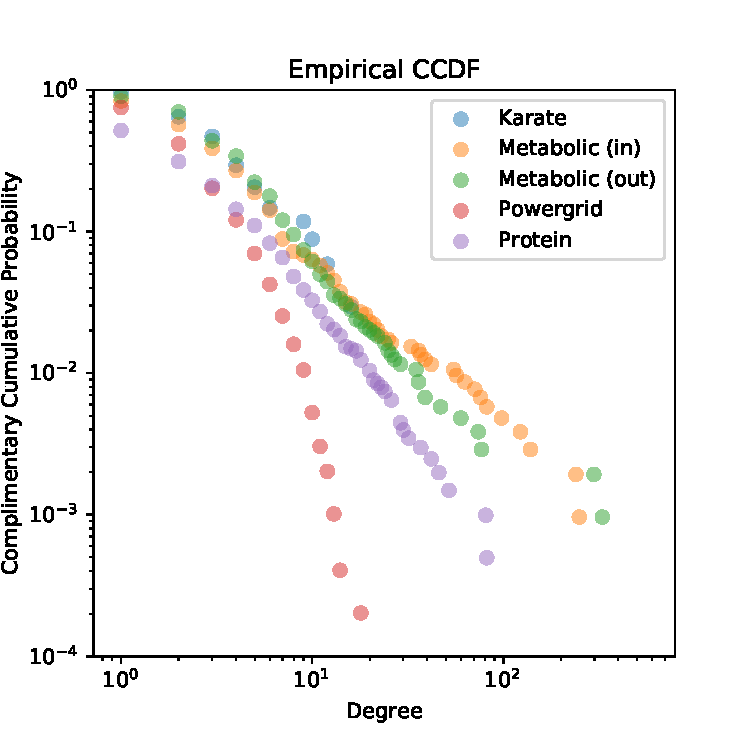
\includegraphics[width=1\linewidth]{degree}
			\caption{Graus - CCDF}
			\label{fig:degree}
		\end{minipage}%
		\begin{minipage}{.5\textwidth}
			\centering
			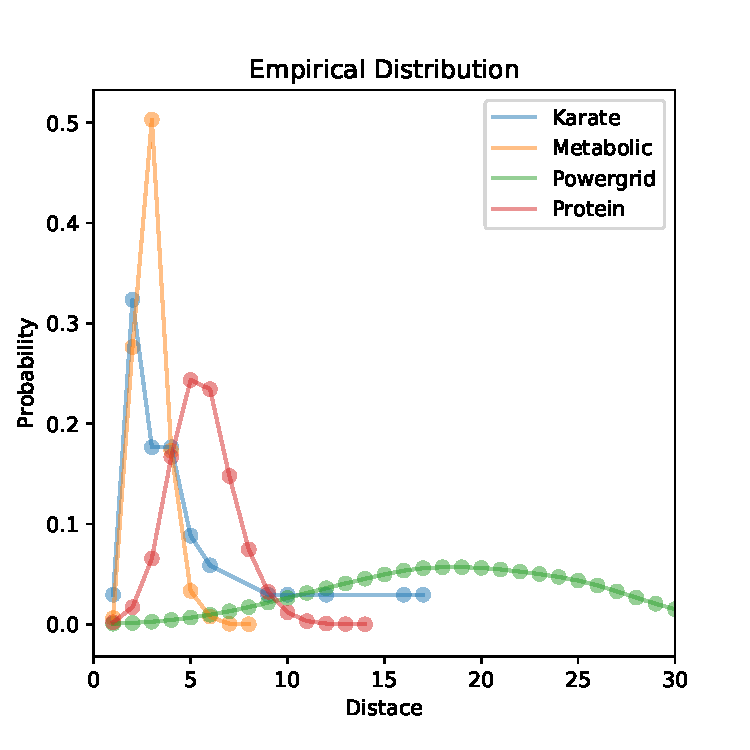
\includegraphics[width=1\linewidth]{distance}
			\caption{Distância - PDF}
			\label{fig:distance}
		\end{minipage}
	\end{figure}

	\begin{figure}[hbt]
		\centering
		\begin{minipage}{.5\textwidth}
			\centering
			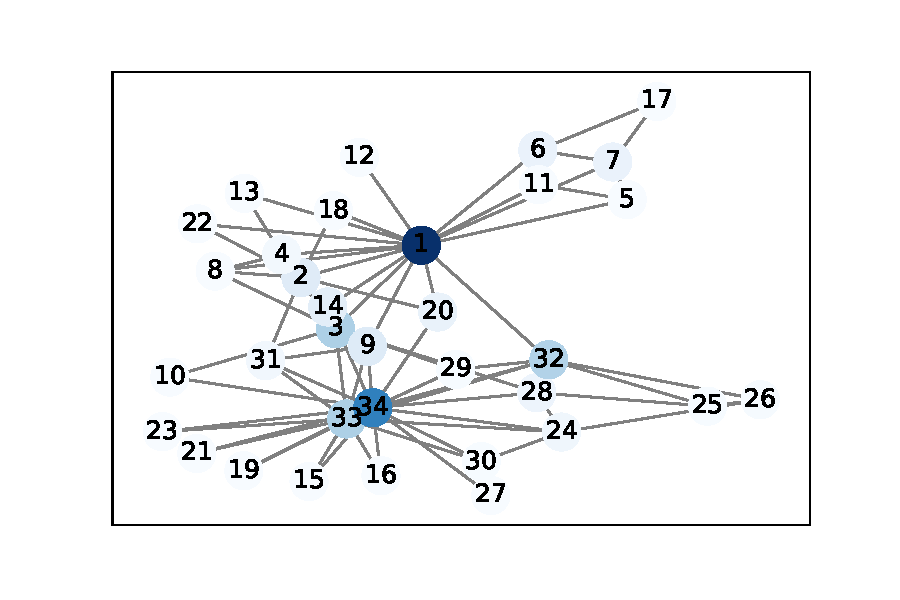
\includegraphics[width=1\linewidth]{karate-betweeness}
			\caption{Karate - Betweness}
			\label{fig:betweeness}
		\end{minipage}%
		\begin{minipage}{.5\textwidth}
			\centering
			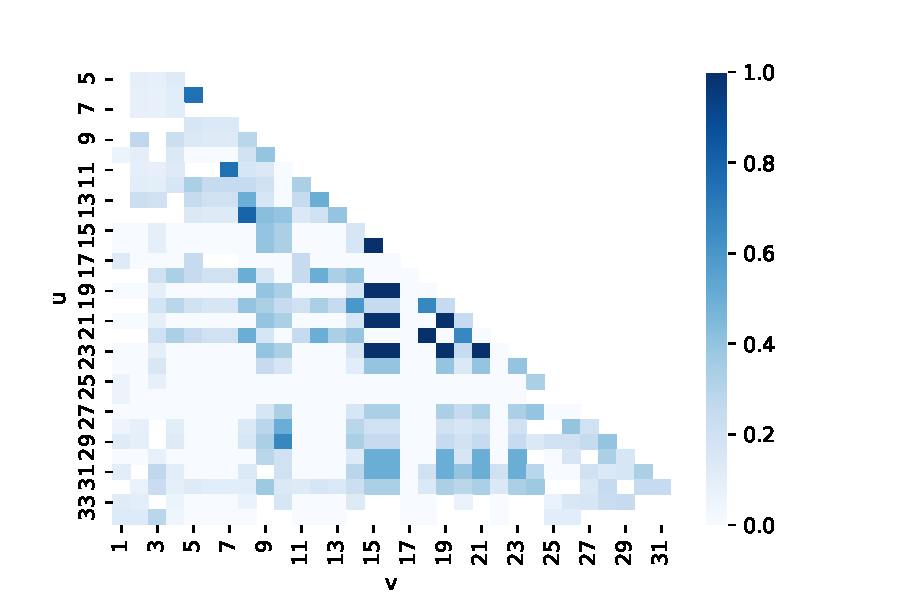
\includegraphics[width=1\linewidth]{karate-jaccard}
			\caption{Karate - Jaccard}
			\label{fig:jaccard}
		\end{minipage}
	\end{figure}
	
	\section{Discussão dos Resultados}
	
	
	Com relação à distribuição de graus, observamos na figura \ref{fig:degree} que as redes Metabolic e Protein possivelmente podem ser modeladas através de uma lei de potência. Já na rede Powergrid, a distribuição claramente não segue uma lei de potência.
	
	Com relação à distância, é interessante observar na figura \ref{fig:distance} que as redes Metabolic e Protein possuem valores de distância esperada próximos, apesar de possuírem características estruturais diferentes. A rede Powergrid, por outro lado, apresenta distância média bem superior às demais redes.
	
	Para a rede Protein, observamos que a maior componente conexa corresponde a 82\% dos vértices da rede, o que corrobora para a característica de ``tudo conectado''.
	
	Com relação à centralidade \textit{Closeness}, verificamos que as redes Karatê e Metabolic apresentam centralidade média maior que as outras duas. Isso é intuitivo, uma vez que a métrica é baseada na distância média de um vértice com o restante do grafo, e as redes PowerGrid e Protein possuem distância média maior. 
	
	Para a Karatê, é possível visualizar a distribuição de \textit{betweeness}, por exemplo, com a coloração dos próprios vértices (\ref{fig:betweeness}). A métrica identifica os vértices mais centrais da rede (1, 34). De fato, sabe-se que os membros 1 e 34 são o gerente e o instrutor do clube. Ainda, a distribuição do índice de similaridade de Jaccard pode ser visualizada através de um mapa de calor (figura \ref{fig:jaccard}), o qual poderia ser utilizado, por exemplo, para identificar possíveis grupos entre os membros do clube.  


\end{document}